\newpage
\section{Implementacion:}
\subsection{Algoritmos:}
\subsubsection{Bubble Sort}
\begin{verbatim}
import time

ruta = 'archivo.txt'

inicio_tiempo = time.time()

with open(ruta, 'r') as archivo:
    datos = archivo.read()

arreglo = list(map(int, datos.split()))

n = len(arreglo)
for i in range(n):
    for j in range(0, n-i-1):
        if arreglo[j] > arreglo[j+1]:
            arreglo[j], arreglo[j+1] = arreglo[j+1], arreglo[j]

with open(ruta, 'w') as archivo:
    archivo.write(' '.join(map(str, arreglo)))

fin_tiempo = time.time()
print(f"Tiempo de ejecución: {fin_tiempo - inicio_tiempo} segundos")
\end{verbatim}
\subsubsection{Counting Sort}
\begin{verbatim}
import time
ruta = 'archivo.txt'
inicio_tiempo = time.time()
with open(ruta, 'r') as archivo:
    datos = archivo.read()
arreglo = list(map(int, datos.split()))

max_valor = max(arreglo)

conteo = [0] * (max_valor + 1)

for numero in arreglo:
    conteo[numero] += 1

indice = 0
for i in range(len(conteo)):
    while conteo[i] > 0:
        arreglo[indice] = i
        indice += 1
        conteo[i] -= 1

with open(ruta, 'w') as archivo:
    archivo.write(' '.join(map(str, arreglo)))

fin_tiempo = time.time()
print(f"Tiempo de ejecución: {fin_tiempo - inicio_tiempo} segundos")
\end{verbatim}
\subsubsection{Heap Sort}
\begin{verbatim}
import time

ruta = 'archivo.txt'

inicio_tiempo = time.time()

with open(ruta, 'r') as archivo:
    datos = archivo.read()

arreglo = list(map(int, datos.split()))

n = len(arreglo)

for i in range(n // 2 - 1, -1, -1):
    indice = i
    while True:
        hijo_izq = 2 * indice + 1
        hijo_der = 2 * indice + 2
        mayor = indice
        if hijo_izq < n and arreglo[hijo_izq] > arreglo[mayor]:
            mayor = hijo_izq
        if hijo_der < n and arreglo[hijo_der] > arreglo[mayor]:
            mayor = hijo_der
        if mayor == indice:
            break
        arreglo[indice], arreglo[mayor] = arreglo[mayor], arreglo[indice]
        indice = mayor

for i in range(n - 1, 0, -1):
    arreglo[i], arreglo[0] = arreglo[0], arreglo[i]  
    tamaño_heap = i
    indice = 0
    while True:
        hijo_izq = 2 * indice + 1
        hijo_der = 2 * indice + 2
        mayor = indice
        if hijo_izq < tamaño_heap and arreglo[hijo_izq] > arreglo[mayor]:
            mayor = hijo_izq
        if hijo_der < tamaño_heap and arreglo[hijo_der] > arreglo[mayor]:
            mayor = hijo_der
        if mayor == indice:
            break
        arreglo[indice], arreglo[mayor] = arreglo[mayor], arreglo[indice]
        indice = mayor

with open(ruta, 'w') as archivo:
    archivo.write(' '.join(map(str, arreglo)))

fin_tiempo = time.time()
print(f"Tiempo de ejecución: {fin_tiempo - inicio_tiempo} segundos")
\end{verbatim}
\subsubsection{Insertion Sort}
\begin{verbatim}
import time

ruta = 'archivo.txt'

inicio_tiempo = time.time()

with open(ruta, 'r') as archivo:
    datos = archivo.read()

arreglo = list(map(int, datos.split()))

n = len(arreglo)
for i in range(1, n):
    clave = arreglo[i]
    j = i - 1
    while j >= 0 and clave < arreglo[j]:
        arreglo[j + 1] = arreglo[j]
        j -= 1
    arreglo[j + 1] = clave

with open(ruta, 'w') as archivo:
    archivo.write(' '.join(map(str, arreglo)))

fin_tiempo = time.time()
print(f"Tiempo de ejecución: {fin_tiempo - inicio_tiempo} segundos")
\end{verbatim}
\subsubsection{Merge Sort}
\begin{verbatim}
import time

ruta = 'archivo.txt'

inicio_tiempo = time.time()

with open(ruta, 'r') as archivo:
    datos = archivo.read()

arreglo = list(map(int, datos.split()))

n = len(arreglo)
sublistas = [[arreglo[i]] for i in range(n)]

while len(sublistas) > 1:
    nuevas_sublistas = []
    for i in range(0, len(sublistas) - 1, 2):
        izquierda = sublistas[i]
        derecha = sublistas[i + 1]
        temp = []
        while izquierda and derecha:
            if izquierda[0] < derecha[0]:
                temp.append(izquierda.pop(0))
            else:
                temp.append(derecha.pop(0))
        temp += izquierda
        temp += derecha
        nuevas_sublistas.append(temp)
    if len(sublistas) % 2 == 1:
        nuevas_sublistas.append(sublistas[-1])
    sublistas = nuevas_sublistas

arreglo = sublistas[0]

with open(ruta, 'w') as archivo:
    archivo.write(' '.join(map(str, arreglo)))

fin_tiempo = time.time()
print(f"Tiempo de ejecución: {fin_tiempo - inicio_tiempo} segundos")
\end{verbatim}
\subsubsection{Quick Sort}
\begin{verbatim}
import time

ruta = 'archivo.txt'

inicio_tiempo = time.time()

with open(ruta, 'r') as archivo:
    datos = archivo.read()

arreglo = list(map(int, datos.split()))

pila = [(0, len(arreglo) - 1)]

while pila:
    inicio, fin = pila.pop()
    if inicio >= fin:
        continue

    pivote = arreglo[fin]
    i = inicio - 1

    for j in range(inicio, fin):
        if arreglo[j] <= pivote:
            i += 1
            arreglo[i], arreglo[j] = arreglo[j], arreglo[i]

    arreglo[i + 1], arreglo[fin] = arreglo[fin], arreglo[i + 1]
    pivote_index = i + 1

    pila.append((inicio, pivote_index - 1))
    pila.append((pivote_index + 1, fin))

with open(ruta, 'w') as archivo:
    archivo.write(' '.join(map(str, arreglo)))

fin_tiempo = time.time()
print(f"Tiempo de ejecución: {fin_tiempo - inicio_tiempo} segundos")
\end{verbatim}
\subsubsection{Selection Sort}
\begin{verbatim}
import time

ruta = 'archivo.txt'

inicio_tiempo = time.time()

with open(ruta, 'r') as archivo:
    datos = archivo.read()

arreglo = list(map(int, datos.split()))

n = len(arreglo)
for i in range(n):
    min_idx = i
    for j in range(i + 1, n):
        if arreglo[j] < arreglo[min_idx]:
            min_idx = j
    arreglo[i], arreglo[min_idx] = arreglo[min_idx], arreglo[i]

with open(ruta, 'w') as archivo:
    archivo.write(' '.join(map(str, arreglo)))

fin_tiempo = time.time()
print(f"Tiempo de ejecución: {fin_tiempo - inicio_tiempo} segundos")
\end{verbatim}
\subsection{Comparaciones:}
\subsubsection{Por Lenguaje}
\textbf{Python}
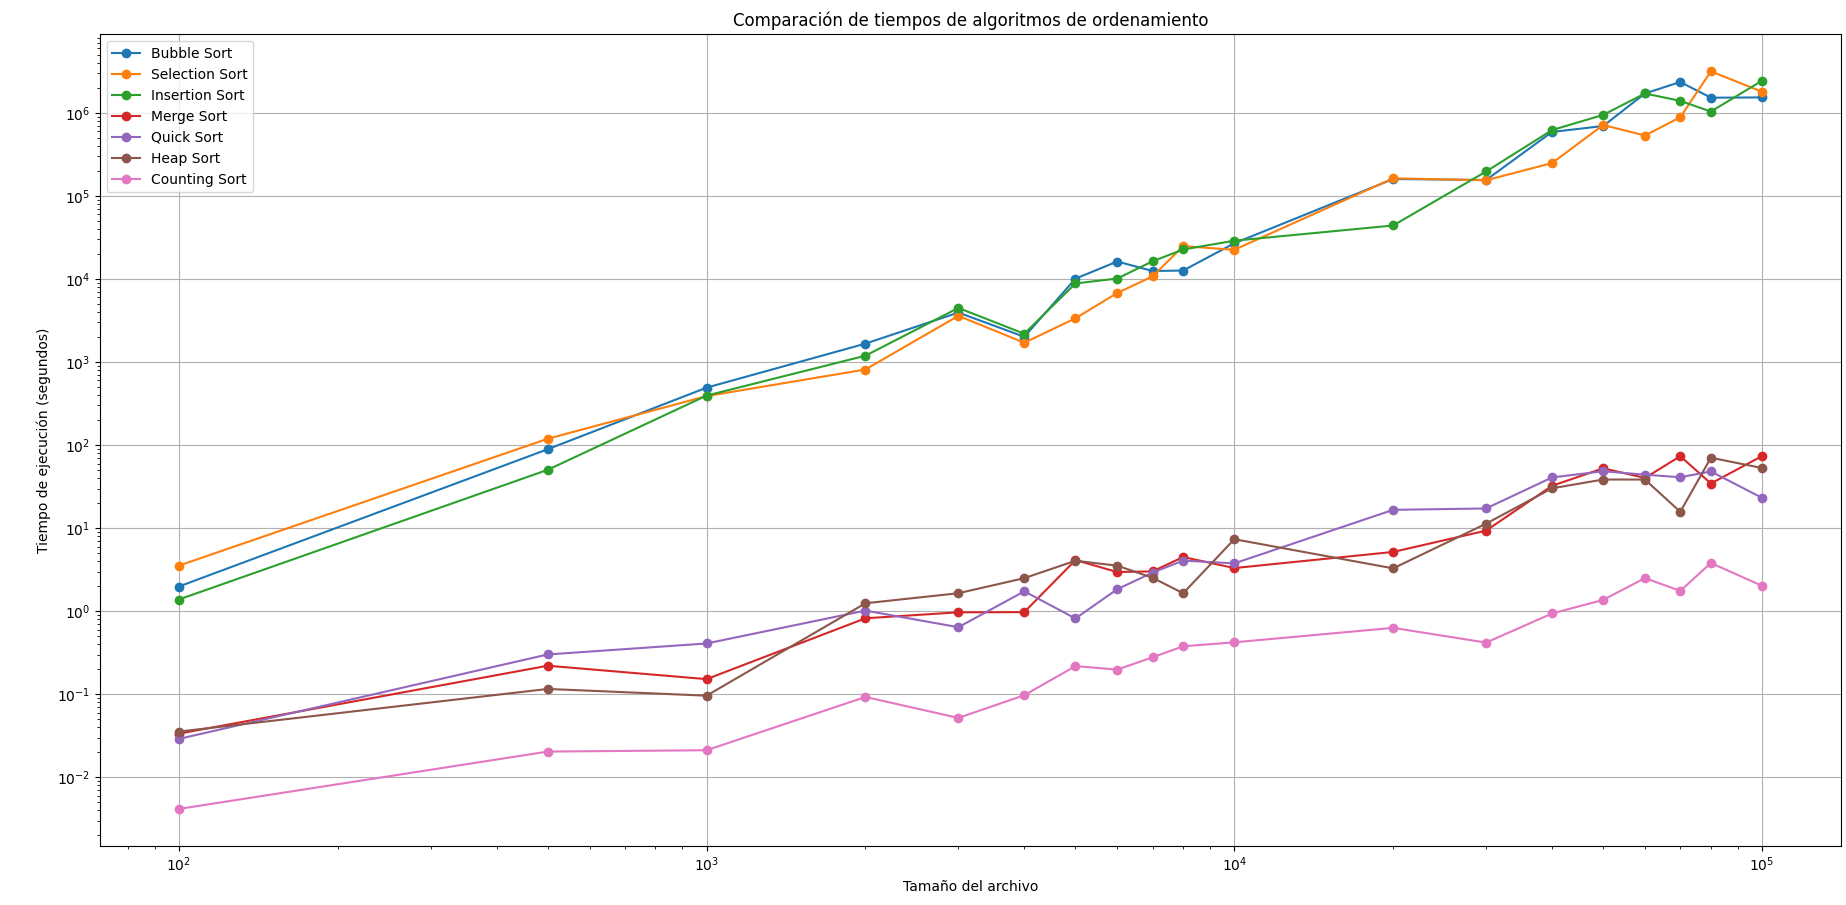
\includegraphics[scale=.25]{img/graficos/por lenguaje/python.png}\\[0.2cm]
\textbf{C++}
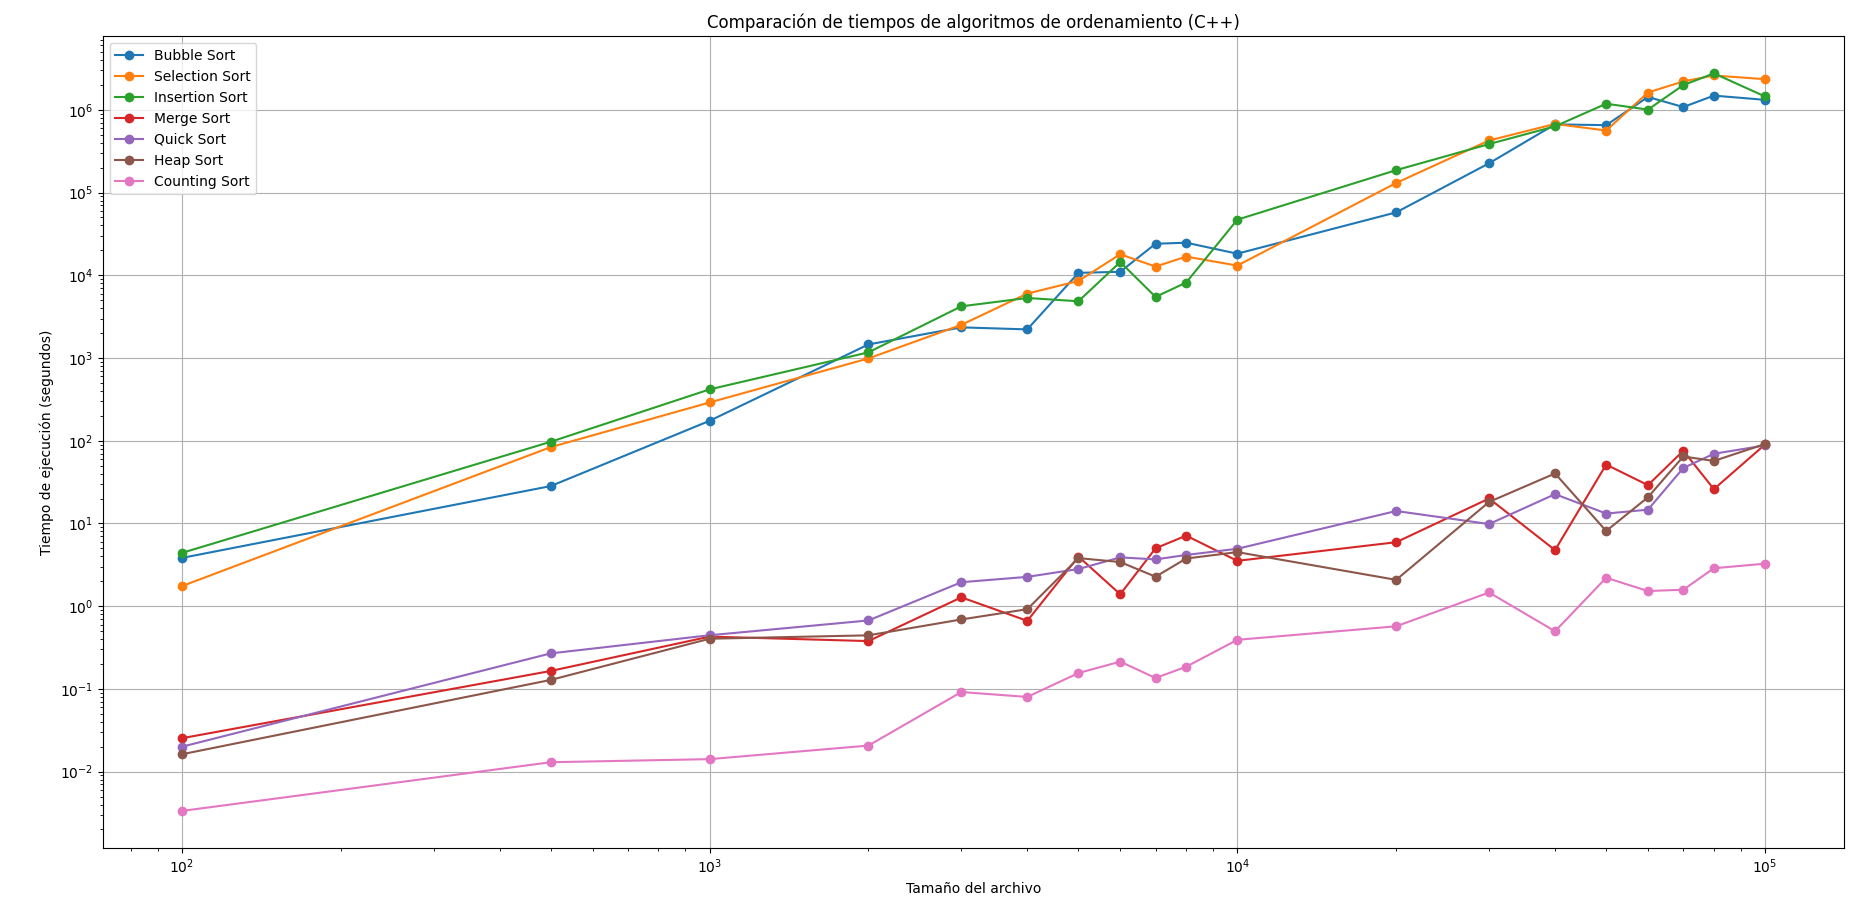
\includegraphics[scale=.25]{img/graficos/por lenguaje/c++.png}\\[0.2cm]
\textbf{JAVA}
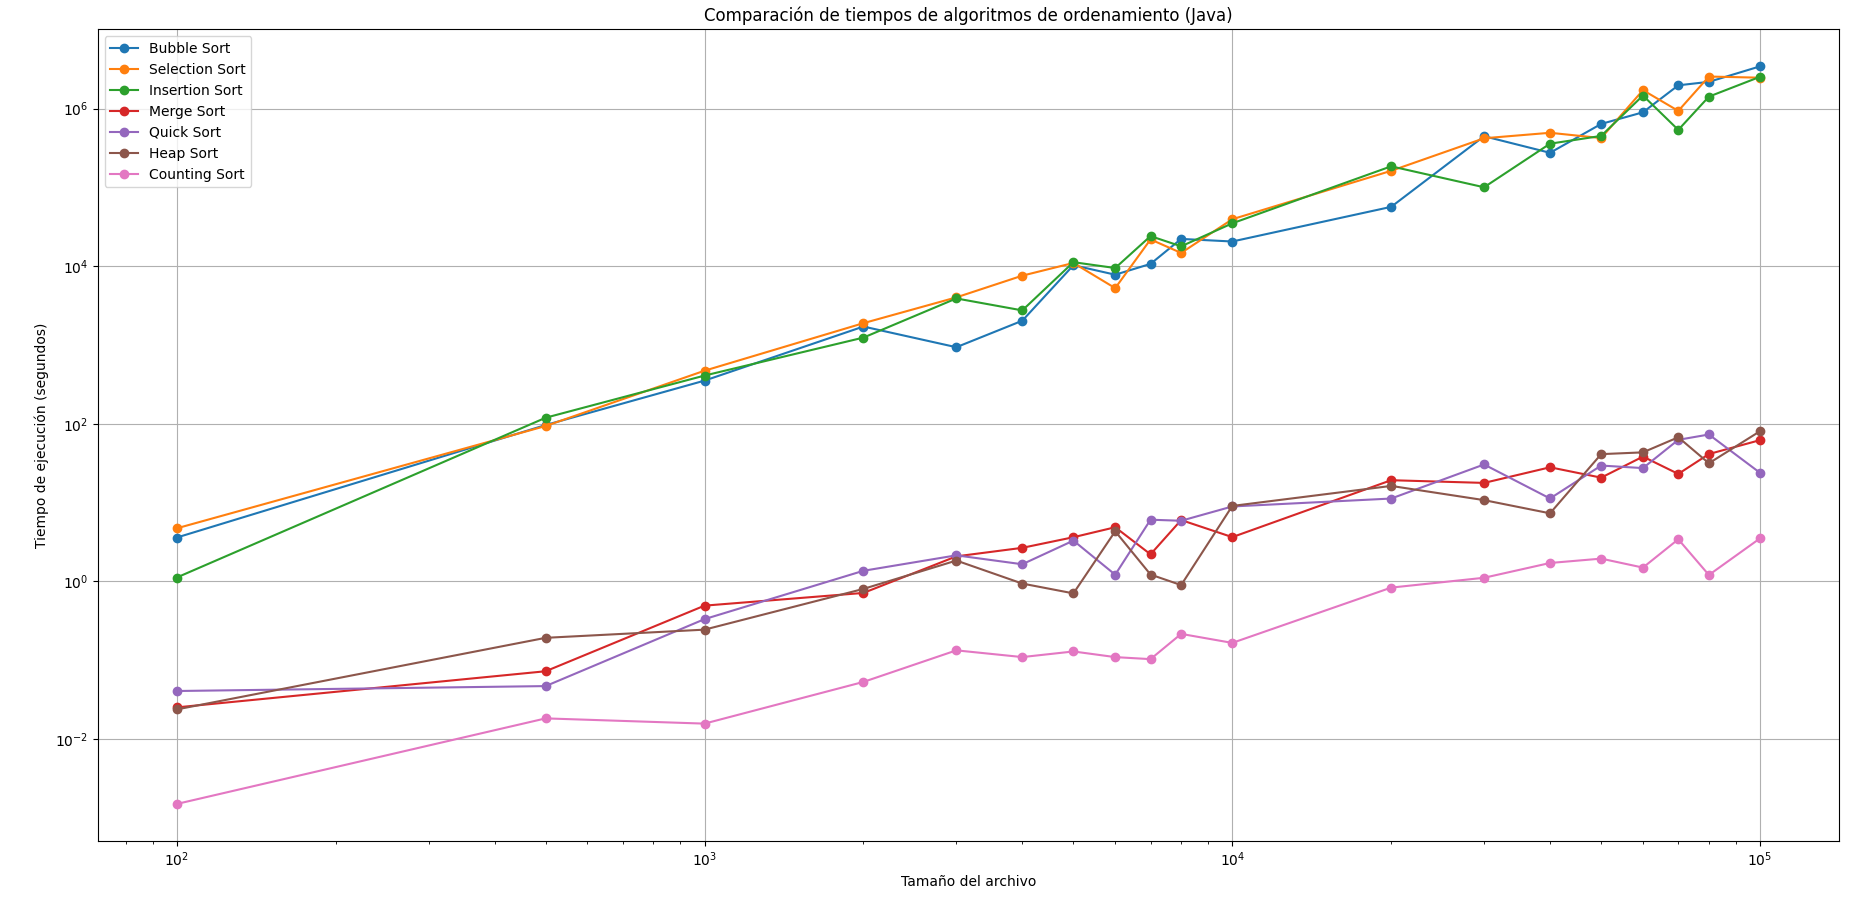
\includegraphics[scale=.25]{img/graficos/por lenguaje/java.png}\\[0.2cm]

\subsubsection{Por Algoritmo}
\textbf{Bubble Sort}
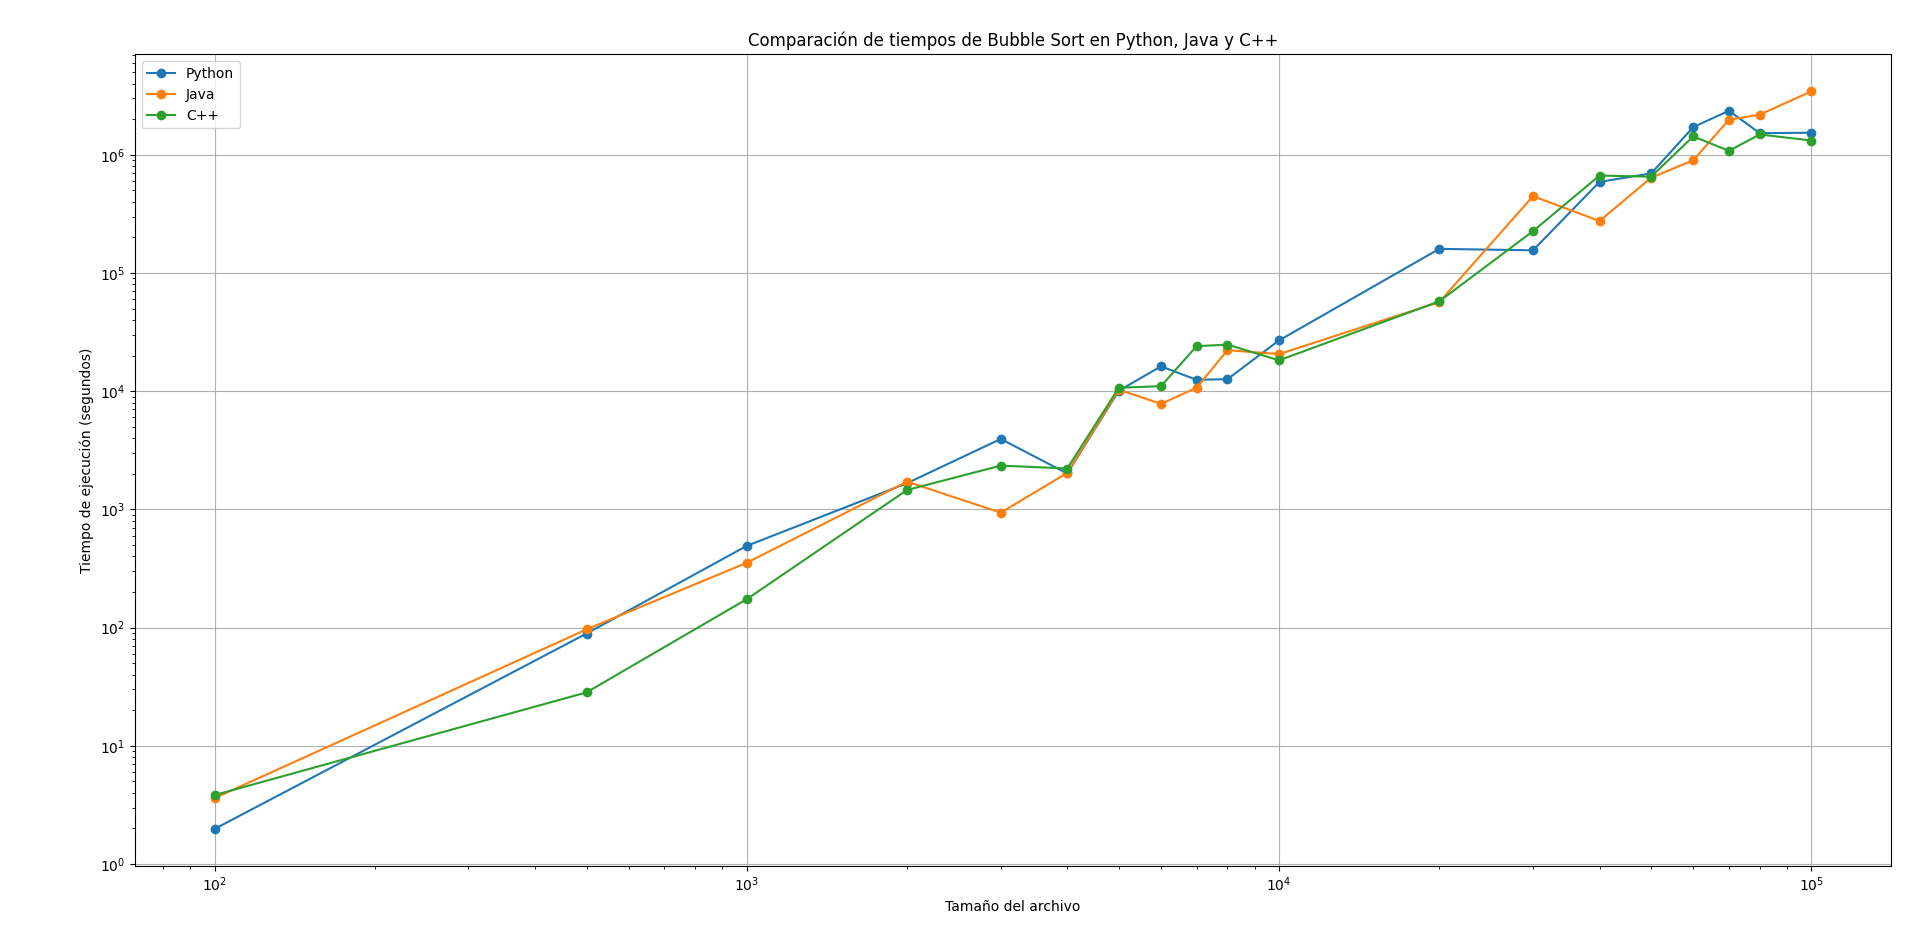
\includegraphics[scale=.25]{img/graficos/por algoritmo/bublesort.png}\\[0.2cm]
\textbf{Counting Sort}
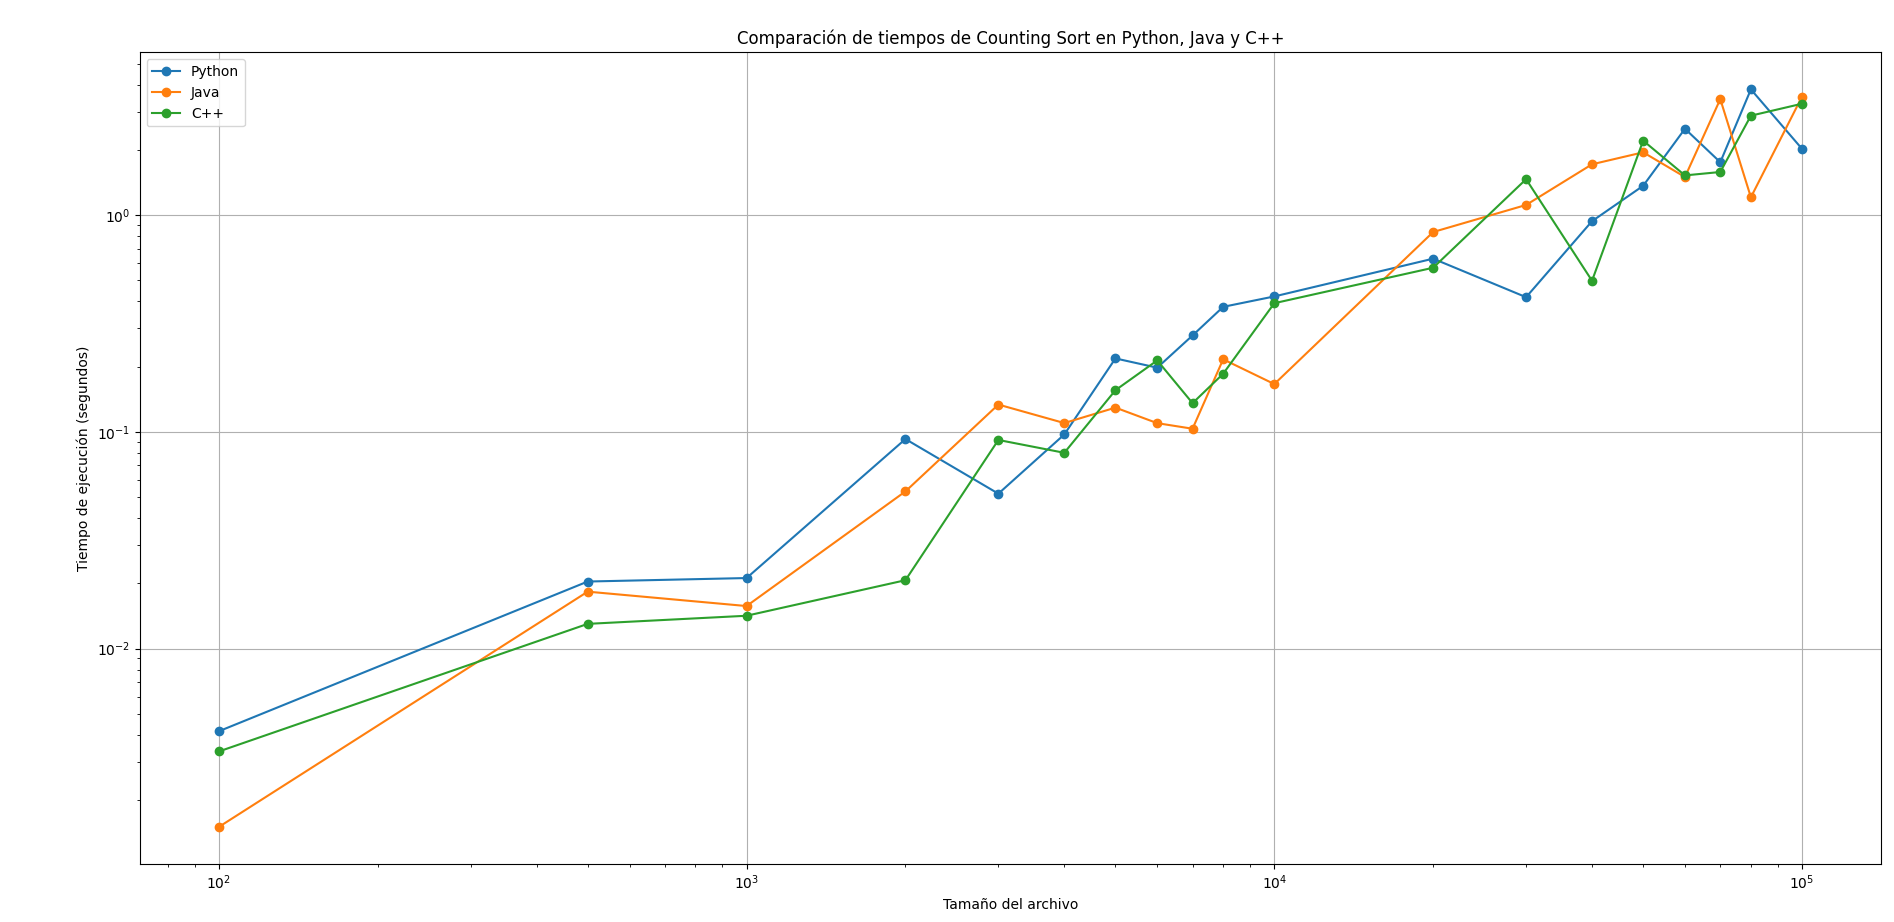
\includegraphics[scale=.25]{img/graficos/por algoritmo/coungtingsort.png}\\[0.2cm]
\textbf{Heap Sort}
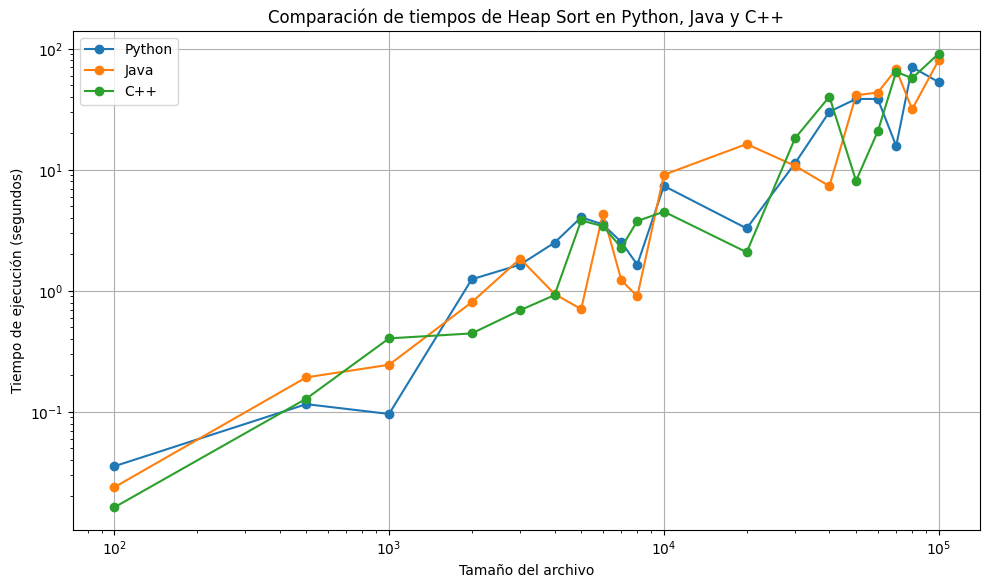
\includegraphics[scale=.25]{img/graficos/por algoritmo/heapsort.png}\\[0.2cm]
\textbf{Insertion Sort}
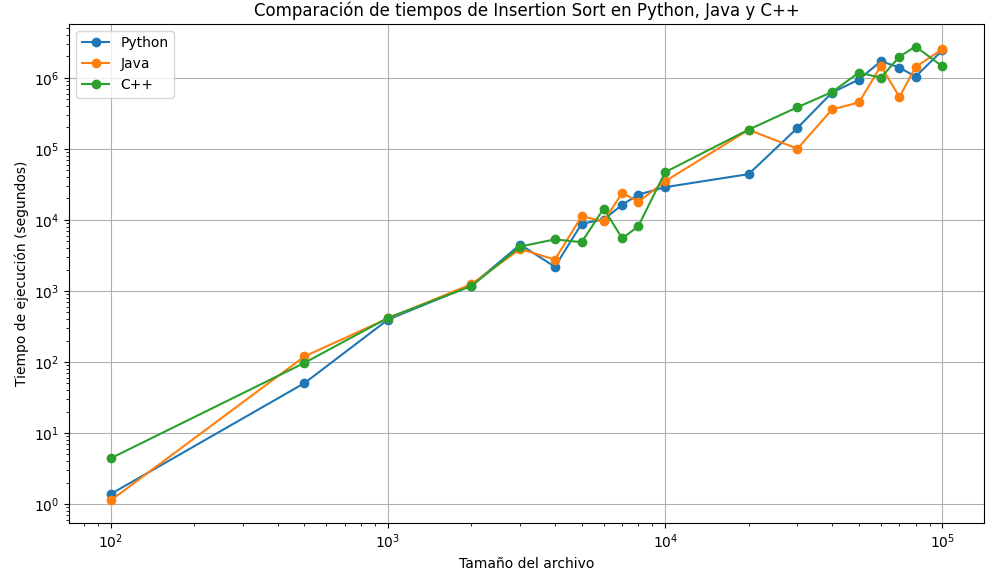
\includegraphics[scale=.25]{img/graficos/por algoritmo/insertionsort.png}\\[0.2cm]
\textbf{Merge Sort}
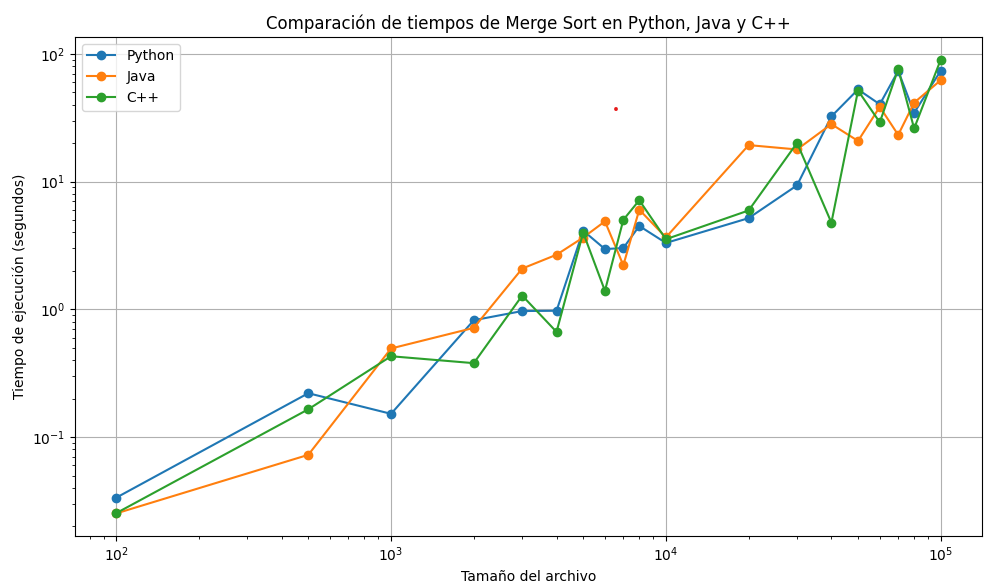
\includegraphics[scale=.25]{img/graficos/por algoritmo/mergersort.png}\\[0.2cm]
\textbf{Quick Sort}
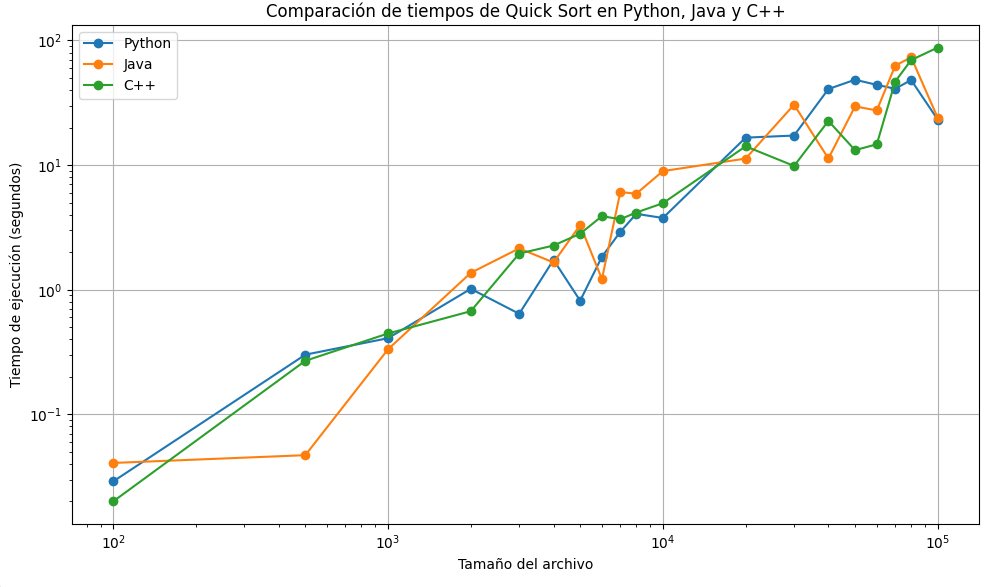
\includegraphics[scale=.25]{img/graficos/por algoritmo/quicksort.png}\\[0.2cm]
\textbf{Selection Sort}
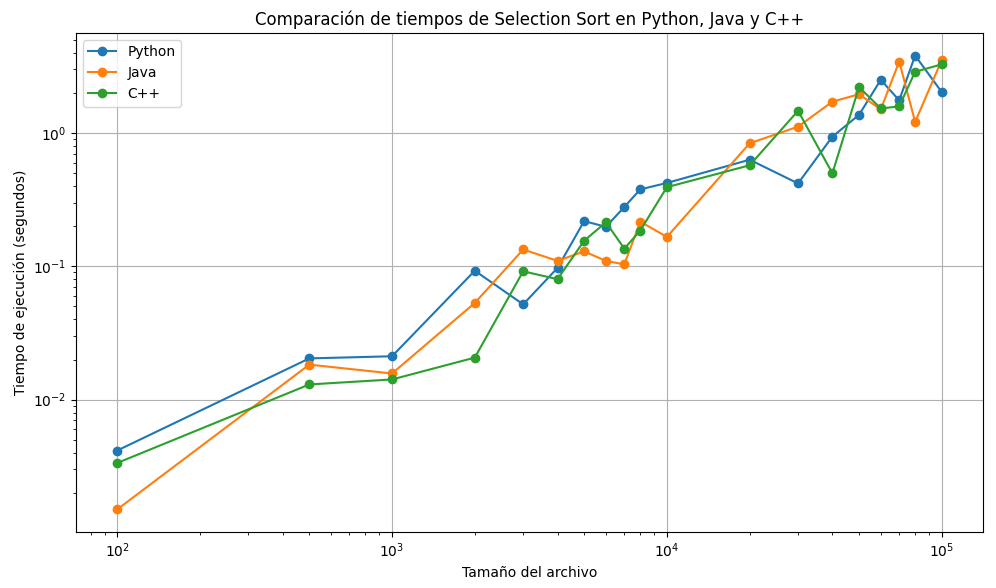
\includegraphics[scale=.25]{img/graficos/por algoritmo/selectionsort.png}\\[0.2cm]